%%%%%%%%%%%%%%%%%%%%%%%%%%%%%%%%%%%%%%%%%%%%%%%%%%%%%%%%%%%%%%%%%%%%%%%%%%%%%%%%
%2345678901234567890123456789012345678901234567890123456789012345678901234567890
%        1         2         3         4         5         6         7         8

\documentclass[letterpaper, 10 pt, conference]{ieeeconf}  % Comment this line out if you need a4paper


%\documentclass[a4paper, 10pt, conference]{ieeeconf}      % Use this line for a4 paper

\IEEEoverridecommandlockouts                              % This command is only needed if 
% you want to use the \thanks command

\overrideIEEEmargins

% Sorts and compresses references properly
% (poor substitute for natbib, but it's the best we can do with this docclass)
\usepackage{cite}

% Give us pretty subfigures
\usepackage{subfig}

% Good math support
\usepackage{mathtools}
\usepackage{amssymb}
\usepackage{graphicx}
\usepackage{caption}
\usepackage{amsmath}
\DeclareCaptionFont{eightpt}{\fontsize{8pt}{9pt}\selectfont #1}
\captionsetup{font=eightpt}

\graphicspath{{figures/}}

% Needed to meet printer requirements.

% See the \addtolength command later in the file to balance the column lengths
% on the last page of the document

% The following packages can be found on http:\\www.ctan.org
%\usepackage{graphics} % for pdf, bitmapped graphics files
%\usepackage{epsfig} % for postscript graphics files
%\usepackage{mathptmx} % assumes new font selection scheme installed
%\usepackage{times} % assumes new font selection scheme installed
%\usepackage{amsmath} % assumes amsmath package installed
%\usepackage{amssymb}  % assumes amsmath package installed


\title{\LARGE \bf
	Learning longer behavioral sequences in a modular robot team  
	to better infer global formation
}    
% Automated synthesis of scalable algorithms for inferring non-local
%properties to assist in multi-robot teaming


\author{Taeyeong Choi, Sehyeok Kang, and Theodore P.~Pavlic % <-this % stops a space
	\thanks{*This work was not supported by any organization}% <-this % stops a space
	\thanks{T.~Choi, S.~Kang, and T. P.~Pavlic are with the School of Computing, Informatics, and Decision Systems Engineering,
		Arizona State University, Tempe, AZ 85281, USA
		{\tt\small \{tchoi4, skang66, tpavlic\}@asu.edu}}%
}


\begin{document}
	
	
	
	\maketitle
	\thispagestyle{empty}
	\pagestyle{empty}
	
	
	%%%%%%%%%%%%%%%%%%%%%%%%%%%%%%%%%%%%%%%%%%%%%%%%%%%%%%%%%%%%%%%%%%%%%%%%%%%%%%%%
	\begin{abstract}
		
		We propose a more powerful machine learning approach, as an extension of \cite{CPR17},
		to tackle the Remote Teammate
		Localization (RTL) problem where a robot member in a multi-robot team is to predict positions
		of all other teammates only using the observations on its nearest neighbor without any
		communication between robots.
		%        In the previous work, we followed a realistic configuration
		%        in which each robot had a limited sensor radius
		%        As each robot had a relatively simple motion rule with dependency on its nearest neighbors,
		In the previous work, we showed feasibility of a scalable method by which
		a predictor robot was trained in a modular 3-robot team but could extend the prediction
		to a larger
		team without additional training, also suggesting an application of such an inference in
		caging mission.         
		In this work, however, we focus mainly on 1) achieving better performance
		to improve the applicability and 2) conducting evaluation in
		more realistic environments. To be specific, we adopt a Long-Short Term Memory (LSTM)
		to learn possible evolution of behaviors in a modular team helping reduce the errors
		from regression outcomes. Furthermore, while the previous work relied only on computer simulations,
		all the experiments here are conducted on a physical two-wheeled robotic platform, \emph{Thymio},
		to demonstrate the performance gain under realistic constraints.
		
	\end{abstract}
	
	
	%%%%%%%%%%%%%%%%%%%%%%%%%%%%%%%%%%%%%%%%%%%%%%%%%%%%%%%%%%%%%%%%%%%%%%%%%%%%%%%%
	
	\section{Introduction}
	\label{sec:intro}
	
	In multi-robot systems including swarms, every robot is usually allowed to observe 
	only a subset of its team members and interact with them to determine the next action 
	according to relatively simple motion rules. 
	Such a property enables the entire system to perform in a distributed manner, and 
	also the behavior of it can be driven easily by a few leader robots to 
	eventually achieve the goal \cite{CPR17, DGRSS17, EB16}. 
	This implies that if a robot has an ability to reognize useful property, e.g.) formation, 
	of the whole team in real time using its local sensors, 
	it could present adjustive actions accordingly to better promote a collective behavior 
	for the sake of the team.
	
	In \cite{CPR17}, we suggested a machine learning method to solve the 
	RTL problem where a robot, called \emph{Tail} at one end of a line formation of 
	a multi-robot team, is to predict positions of all other teammates only using local
	observations about a single nearby teammate. Since each robot has a limited sensor
	radius and a relatively simple motion rule with dependency 
	on the position of its nearest neighbors, 
	the \emph{Tail} has to be able to learn the regularity 
	of the observed motions of neighbor to finally infer the poses of all other robots.
	We introduced a repetitive prediction scheme to use predictions on 
	nearer teammates to make predictions on farther ones until the prediction 
	reached the \emph{Head} robot at the other end in line formation. 	
	Also, computer simulations showed the feasibility of the method 
	especially with caging scenario in which the \emph{Tail} could recognize a
	caging action of \emph{Head} in early stage and promote a proactive maneuver to 
	better assist in team cooperation. 
	
	RTL problem provides some unique characteristics compared to general localization problems. 
	In RTL, the robot does not execute predictions on its own location but on  
	its teammates using accessible information.
	Moreover, the robot is not allowed to communicate with other members during 
	prediction phase to consider communication-free scenarios, which differs from 
	cooperative localization problem. 
	Hence, RTL usually assumes that robots behave with correlations with their neighbors 
	so that the resulting behaviors contain cues about the state of their neighbors. 	
	In this sense, state observers in networked robotic system could be a more similar 
	configuration to RTL, but RTL more emphasizes 
	scalable applications to variable sizes of robot team as well as a general framework 
	that would impose little constraint on dynamics of the system.
	
	%
	\begin{figure}\centering
		\includegraphics[width=1.\columnwidth]{fig_Concept}
		\caption{Illustration of our proposed pipepline in a snapshot example of 
			$5$~robots at time $t$.
			Each robot has a limited view and a motion rule dependent on its neighbors
			except the \emph{Head} robot leading the team at the front. 
			\emph{Tail} uses recent observations on its neighbor, \emph{Follower 3}, 
			which is denoted as $O(t-1,t)$. A sequence of historical poses, $h$, is 
			also encoded for the model to make a final prediction on the 
			unseen teammates. 
		}
		\label{fig:Concept}
	\end{figure}
	%
	
	Figure~\ref{fig:Concept} illustrates our proposed pipeline in which 
	a deep neural network is to learn to synthesize the observations on its neighbor 
	with knowledge about historical positions of all the teammates. 
	As shown in Fig.~\ref{fig:DL_Pipeline}, a LSTM layer is deployed to encode 
	the historical sequence input, which could learn probable evolution of the 
	team shape over time under physical constraints. 
	The sequence encoding could help filter out impossible solution candidates
	that the model might produce if it only utilized the recent observations on 
	the neighbor, as in \cite{CPR17}, 

	Not only a more powerful model but also a more realistic experiment 
	environment are prepared. Previously, we 
	conducted all demonstrations on computer simulations, but in this work, 
	a physical two-wheeled robotic platform, \emph{Thymio} \cite{Shin14}, is mainly 
	used to set up more realistic environments.
	
%	All codes are available online\footnote{http://www.github.com/ctyeong}, and supplementary videos 
%	are submitted as well. 
		
	This paper is organized as follow. 
	In Section~\ref{sec:related_work}, we explore related literature and the distinction of our work. 
	Section~\ref{sec:problem_description} explains more details about our setting of RTL problem. 
	Then, we introduce our method, \emph{IPY-Net}, in Section~\ref{sec:method}, and 
	Section~\ref{sec:experiments} explains details about experiments performed on real robots, 
	including data collection, hyperparameters used for learning, and the results. 
	Lastly, we summarize our research and discuss future directions 
	in Section~\ref{sec:discussion_and_future_work}.

	%
	\begin{figure}\centering
		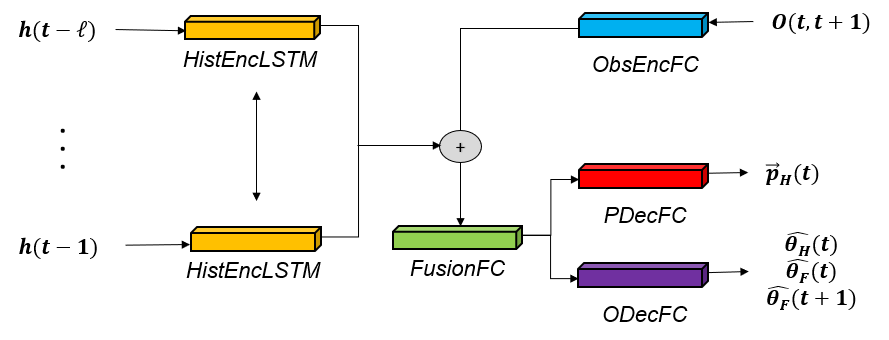
\includegraphics[width=1.\columnwidth]{fig_DL_Pipeline}
		\caption{Structure of our proposed deep neural network. 
			This is an snapshot example when applied to a focused module of
			$3$~robots, called \emph{Tail, Follower, Head} within it, at time $t$. 
			The Encoder-Decoder structure encodes
			1) historical positions and orientations of \emph{Follower} and \emph{Head} 
			until $t-2$ and 2) the observed positions of the \emph{Follower} at $t-1$ and $t$. 
			The decoder part learns to estimate 1) the position of \emph{Head} at $t-1$ and 
			2) orientations of \emph{Follower} at $t-1$ and $t$ and \emph{Head} at $t-1$.   
		}
		\label{fig:DL_Pipeline}
	\end{figure}
	%
	
	
	\section{Related work}
	\label{sec:related_work}
	
	Although the RTL problem is to localize robots, as mentioned in Sec.~\ref{sec:intro}, 
	it has unique properties compared to traditional localization problems including
	cooperative localization or tracking \cite{LSRB16, FSDO10, CX14, DMG15}. Rather, 

	\subsection{Group state recognition}
	\label{sec:group_state_recognition}
	Our approach is basically an attempt to infer positional state of the entire 
	multi-robot team, using only locally obtainable information in the aspect of a robot 
	member. This is because the knowledge about global configuration could 
	help make a better decision for the sake of whole team. In this spirit, 
	the authors in \cite{BG14, BSB16} sampled a subset of robot agents from a swarm to 
	monitor their local interactions and classify the swarm-level behavior. 
	In fact, they implemented relatively simple robots run on a virtual simulator and 
	predefined selections of global behaviors such as \emph{flock} and \emph{torus}. 
	In contrast, our work is to estimate pose of real robots, which would require a more 
	powerful model to regress on any value in a wide range of arena size. 

	\subsection{Behavioral cue interpretation}
	\label{sec:behavioral_cue_interpretation}
	
	One of the main assumptions in RTL is the simple motion rule of each robot which 
	has dependency on the state of its neighbors. This implies that the behavior of 
	neighbors could be a method to encrypt the state change of more remote teammates.
	In \cite{NPCBW12, DCV16}, Novitzky at el. and Das et al. employed a type of
	special action, which appeared like "waggle dance" of honeybees \cite{VonFrisch67}, 
	in robot team so that the behavior could convey a meaning between robots. 
	Our work also encourages a robot to decode behavioral cues, but it occurs without 
	entering an explicit phase of signaling. In other words, the robot has to learn 
	to gain useful information from a sequence of continuous usual interactions. 	
	
	\subsection{Robot dynamics learning}
	\label{sec:robot_dynamics_learning}
	
	Byranvan and Fox in \cite{BF17} proposed a deep learning approach 
	to predict the next visual frame given a current frame and the information 
	of force that would affect one of the shown objects. One of their examples was 
	to understand the dynamics of robotic arms and the relationship with control 
	commands possibly executed. In the RTL problem also, the \emph{Tail} robot may 
	have known 
	a global shape of robot team, and it has to be able to predict the future 
	formation as a new observation on its neighbor is provided, which would encode 
	the information of an unseen force driving the team. Such a similarity inspired 
	the architecture of our neural network model, but they focused on learning 
	motions of rigid objects, while a chain of robots in our work can present 
	much flexibility in team shape. In addition, the force is inferred by 
	movements of the neighbor, which would likely contain noise to some level, while 
	\emph{SE3-Nets} is provided with clear information about the applied force.  
	
	This work is an extension of our previous work in \cite{CPR17} in which 
	the configurations for RTL problem were first introduced with realistic assumptions. 
	To solve the problem particularly with little communication, 
	the \emph{Tail} robot is designed to use a repetitive strategy of inference 
	with which the predictions on a closer robots are used as input to 
	prediction for more distant team members. Such an approach enables to scale 
	up the prediction capability without further training as more robots are added.
	Albeit we use the same prediction scheme with repetition, here we focus 
	more on developing a more powerful regressor to broaden applicability and 
	also demonstrating the performance in a multi-robot team implemented on 
	real robotic platform. 
	
	
	\section{Problem Description} 
	\label{sec:problem_description}
	
	Basically, we follow the problem configurations for remote teammate localization introduced in 
	\cite{CPR17}. A robot team moves in a line formation in which	each robot has 
	two adjacent neighbors except for the ones at both ends, each of which has only one neighbor. 
	The robot on one end is the only robot that tries to move to a 
	predetermined destination independent from its neighbor. The robot is called 
	\emph{Head}, and the robot on the opposite end is named \emph{Tail}. 
	All the robots in-between are \emph{Follower}~$i$ where $i \in \{1, 2, ..., n-1\}$ starting
	from the robot closest to the \emph{Tail}.
	
	All the robots are set to take actions as formulated in \cite{CPR17} leading  
	the \emph{Follower} robots and the \emph{Tail} to behave based on the 
	current positions of their close neighbors. As will be explained in 
	Section~\ref{sec:experiments}, we utilize the computational, sensory capacity of a central 
	computer in experiments. Therefore, technically the global positions are used to calculate the next 
	spatial destination of each robot, and then the formula in [] helps generate an actual motion 
	command to operate two wheels to change its pose according to nonholonomic kinematics. 
	
	The remote teammate localization is to localize all the teammates in the view of 
	\emph{Tail} only using locally visible information, which is the position of 
	\emph{Follower}~$1$ at every time step. We assume that until a specific time instant 
	$t$, all the information about positions and orientations of all robots 
	were shared with the \emph{Tail} robot, but from $t+1$, such information is no longer 
	available causing a need of the localization approach utilizing local observations.	
	This may simulate some realistic scenarios where 
	an external technical issue occurs at some time point disabling the information 
	transfer, or the robot team intentionally stops the communication at some regions for security 
	or for saving on the cost.
	 
	
	\section{Method}
	\label{sec:method}
	
	We refer to the inference scheme of our previous work \cite{CPR17} in which 
	a regressor is trained in a short line of $3$ robots, and when employed for a larger team, 
	relaying pose estimations are performed along with the chain of $3$-robot modular teams. 
	
	delay, 


	\subsection{Imaginative representation} 
	\label{sec:imaginative_representation}
	
	\emph{IPY-Net} is designed to produce probabilistic prediction outcomes that contain 
	uncertainty to some level. Specifically, the training process is to encourage to learn 
	the probability distribution on predicted position or orientation. 
	Furthermore, during relaying prediction, the model has to be able to understand 
	the probability distribution predicted at a previous $3$-robot module to 
	make prediction for the current one.  
	
	To be specific, \emph{IPY-Net} adopts a $m \times m$ matrix, which is an image, and 
	a $1 \times k$ matrix to represent position and orientation, respectively. Because  
	each matrix is a probability distribution, the summation of all elements must be $1$. 
	For example, an observed $x$ coordinate is first converted by Equation~\ref{eq:x_conversion}.
	
	\begin{equation}
	\label{eq:x_conversion}
		x' = \frac{x - x_{min}}{x_{max} - x_{min}} \times m - \frac{m}{2}
	\end{equation}
	
	where $x_{min}$ and $x_{max}$ are the minimum and maximum of $x$ coordinates
	empirically observed. $y'$ can be calculated from a $y$ coordinate in a similar way. 
	Then, the position matrix $M_p$ initialized with zeros is updated 
	
	\begin{equation}
		\begin{aligned}
		M_{p}(\lfloor{x'}\rfloor, \lfloor{y'}\rfloor) \\
		M_{p}(\lfloor{x'}\rfloor+1, \lfloor{y'}\rfloor) \\
		M_{p}(\lfloor{x'}\rfloor, \lfloor{y'}\rfloor+1) \\
		M_{p}(\lfloor{x'}\rfloor+1, \lfloor{y'}\rfloor+1) 
		\end{aligned}
	\end{equation} 
	
	We use the image representation, since it allows to learn an arbitrary probability distribution 
	instead of a known distribution constrained on a set of parameters.
	
	
	\subsection{IPY-Net pipeline}
	\label{sec:ipy-net_pipeline}
	 
	
	
	\section{Experiments} 
	\label{sec:experiments} 
	
	
	\begin{table}[t]
		\label{table:data_description}
		\centering
		\begin{tabular}{|c|c|c|c|c|}
			\hline
						&  Duration & Num. of Samples & Num. of Instances  \\ \hline
			$3$ robots & $100.6$ minutes & $6,975$ & $465$  \\ \hline
			$5$ robots & $45.0$ minutes  & $3,120$ & $208$  \\ \hline
		\end{tabular}
		\caption{Description of data collected from executions of $3$-robot and $5$-robot teams.}
	\end{table}

	\begin{table}[]
		\label{table:overall_performance}
		\centering
		\begin{tabular}{|c|c|c|}
			\hline
			&  $3$ robots & $5$ robots  \\ \hline
			Avg Distance & $20.0$ & $30.0$  \\ \hline
		\end{tabular}	
		\caption{Description of data collected from executions of $3$-robot and $5$-robot teams.}
	\end{table}
	
	
	To demonstrate the effectiveness of our method, we employ a physical robotic platform, 
	\emph{Thymio} \cite{Shin14}, which allows to execute a team of small two-wheeled mobile robots.   
	We use a central computer connected with a overhead camera to simulate better proximity 
	sensors, a more powerful computing power, and a GPS system that would easily run on each robot in 
	real scenarios. The central system is set up to detect the locations of robots in real time 
	and communicate with a \emph{Raspberry Pi} board \cite{Upton14} on each robot to send
	the next command relying on its neighbors. Although the experiment configuration involves 
	such external computations and sensors due to limited capability of \emph{Thymio}, 
	most of realistic assumptions hold, and the robots are still influenced by 
	physical constraints and disturbance in motion. For better understanding of readers, 
	we submit a supplementary video. 
	
	The location detection is performed at $4$ frames per second at each of which 
	a new command is received by each robot. Also, 
	all coordinates and orientations at $2$ frames per second are collected, which 
	is not necessarily synchronized with the command timing. 
	
	Two different sizes of robot team are deployed throughout following experiments: 
	$3$~robots and $5$~robots in which the \emph{Head} robot continues to receive a command to 
	move to an arbitrary destination point nearby in a $OO \times OO$ meters arena. 
	Table~\ref{table:data_description} shows details about the data collected from 
	each configuration where a sample refers to a set of coordinates and orientations recorded 
	at an instant time step, and an instance is a sequence of samples for $13$ seconds. 
	The instances are clustered to have at least $7$-second time gap to another so that
	the motions between separate ones have only little dependency. 
	
	$70$\% data from the $3$-robot team is used to train \emph{IPY-Net} by feeding each sample, 
	and the rest $20$\% is used for test. 
	The trained model is also tested with the $5$-robot team, in which the relay prediction is 
	initialized at the beginning of each instance. 
	The length of history is set to $5$~seconds to accept inputs for past $10$~time steps, and 
	the predictions occur for the next $8$~seconds.  
	 	
	\emph{IPY-Net} is implemented in \emph{Tensorflow} \emph{Python} library \footnote{https://www.tensorflow.org/} 
	to realize the entire pipeline. The evaluation is reported in Euclidean distance between 
	the predicted position and the truth, using the model that achieves the best performance 
	during $100$ epochs, by which the loss mostly converges to zero. 

	We compare our proposed model to four different approaches such as: 
	\begin{itemize}
		\item \emph{$2$X Heuristic}: 
		The prediction on \emph{Head} within a modular team is performed by doubling the vector 
		$\vec{p}_{F} - \vec{p}_{T}$.
		
		\item \emph{FC}: 
		Two fully connected layers run in the predictor without considering historical 
		information, which is based on \cite{CPR17}.  
				
		\item \emph{LSTM-FC}: 
		Model combining the historical LSTM and FC layers similar to \emph{IPY-Net} except that 
		all inputs and outputs are represented as numerical values instead of images. 
		
		\item \emph{I-LSTM-FC}: 
		Imaginative model using the same structure as \emph{IPY-Net} with difference that 
		only best predictions on coordinates or orientation are preserved from each predicted image. 
		As needed, the preserved information is processed to generate a new image input during 
		relay prediction process.
	\end{itemize}	

%	\subsection{Data collection} 
%	\label{sec:data_collection}
	
	
%	\subsection{Results} 
%	\label{sec:results}

	\begin{figure}[t]
	\centering
	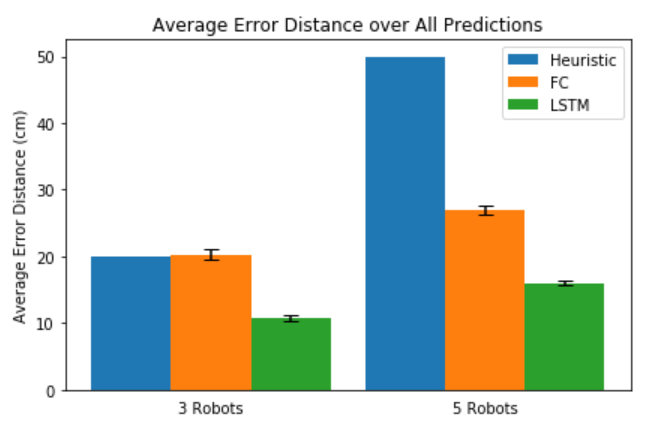
\includegraphics[width=1.\columnwidth]{fig_macro_eval}
	\caption{Prediction errors of \emph{IPY-Net} and \emph{I-LSTM-FC} 
		for different robots at each time step.  
	}
	\label{fig:macro_eval}
	\end{figure}


	\begin{figure}[t]
		\centering
		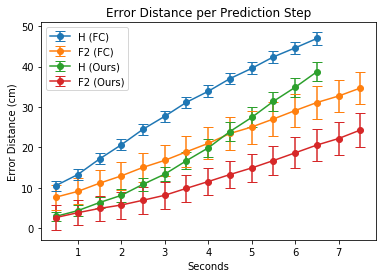
\includegraphics[width=1.\columnwidth]{fig_micro_eval}
		\caption{Prediction errors of \emph{IPY-Net} and \emph{I-LSTM-FC} 
			for different robots at each time step.  
		}
		\label{fig:micro_eval}
	\end{figure}

	
	\subsection{Overall accuracy}
	\label{sec:overall_performance}
	
	We show overall performance of each model in Table~\ref{table:overall_performance}. 
	The error distance is averaged for all samples of all robots. 

	
	\subsection{Microscopic analysis}
	\label{sec:microscopic_analysis}
	
	Here, we further analyze the behaviors of top two models in overall performance 
	by focusing more on errors for different robots at each time step. 
	The robot-wise error is averaged at each step across instances. 
	The result could help compare the upper bounds of errors of the models and 
	understand the feasibility of them during the instance interval. 

	
	\begin{figure*}[t]
		\centering
		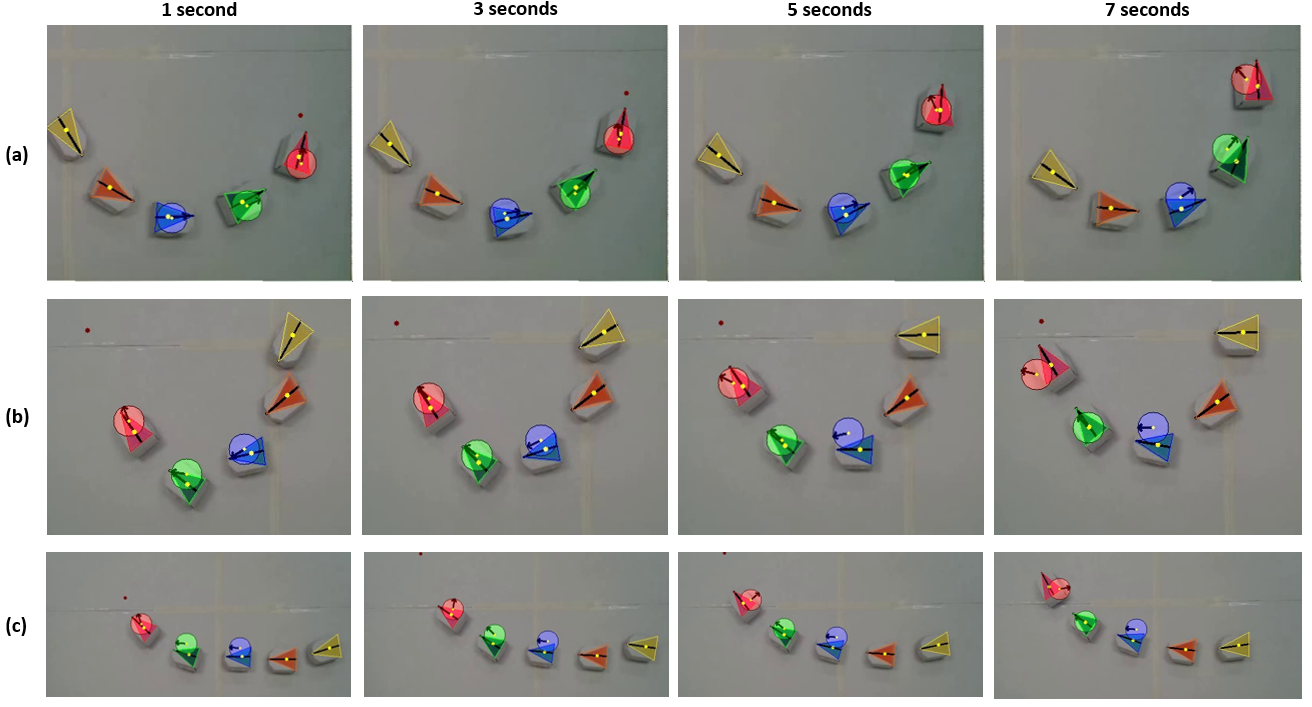
\includegraphics[width=1.8\columnwidth]{fig_preds}
		\caption{Visualized predicted heatmap examples generated from \emph{IPY-Net}. 
			Each row contains snapshots of three instant time steps during a unique 
			instance. In each instance, the frames are sorted in increasing order in time. 			 
		}
		\label{fig:preds}
	\end{figure*}

	
	\subsection{Qualitative results} 
	\label{sec:qualitative_results} 

	This section visualizes the prediction outcomes of \emph{IPY-Net}, while the robot team
	evolves its shape over time. Figure~\ref{fig:heatmap} displays three separate instances in which 
	the generated heatmaps are overlaid on the corresponding original video frames illustrating 
	the predicted probability distribution of the team-level formation. 
	
	The results imply that \emph{IPY-Net} can properly track the emerging behaviors of the team 
	triggered by arbitrary motion sequences. Moreover, the visualized output helps
	human users better interpret the outcome taking into consideration the confidence levels 
	offered by the predictive model. 
	

	\section{Discussion \& Future work}
	\label{sec:discussion_and_future_work}
	
	We have shown \emph{IPY-Net}, a powerful approach to tackle the remote localization problem 
	where a robot with limited sensors is to predict positions of all others only using 
	observations about its nearest neighbor. 
	\emph{IPY-Net} follow the fundamental spirit of \cite{CPR17} to apply a predictor 
	trained for a small robot team to a chain of them in a larger team, since it 
	can provide a scalable feature without re-training.   
	The distinction in \emph{IPY-Net} is , however, to use a sequence of historical knowledge and 
	make predictions based on imagination of robot states including position and orientation.
	We expected learning with history would help regulate the model on physical constraints on 
	the team formation, and also the imaginative representation could contain 
	certainty about the prediction, which would bring about more robust performance. 
	
	The experiment results were obtained using a realistic robotic platform to prove 
	that our method outperforms not only the regressor
	introduced in \cite{CPR17} but also a general state-of-the-art neural network 
	model that is able to use historical data. Especially, our model can present 
	stable performance even when the input contains some errors which have occurred in 
	previous prediction. 
	  
	
	In future work, 
	
	
{\small
	\bibliographystyle{IEEEtran}
	\bibliography{IEEEabrv, IEEEexample}
}


\end{document}
